\section{Анализ задания}

В рамках данного курса необходимо разработать простое приложение, позволяющее продемонстрировать основные архитектурные принципы 
проектирования программного обеспечения с использованием технологии Enterprise Java Beans (EJB). В качестве системы рассмотрим систему 
управлению персоналом, позволяющую автоматизировать некоторые аспекты повседневной деятельности работников компании. На этапе проектирования 
такой системы были выделены следующие роли и их интересы:

\begin{itemize}
    \item Работник 
    \begin{itemize}
        \item Сообщать время своего отсутствия в офисе.
        \item Резервировать время отпуска. 
    \end{itemize}
    \item Менеджер
    \begin{itemize}
        \item Имеет те же интересы, что и работник.
        \item Одобрять/отклонять запросы закрепленных за ним работников.
        \item Выписывать премию любому закрепленному за ним работнику. 
    \end{itemize}
    \item Бухгалтер
    \begin{itemize}
        \item Имеет те же интересы, что и работник.
        \item Одобрять/отклонять премию, выписанную работнику, закрепленному за ним.
    \end{itemize}
\end{itemize}

Используя эти данные, построим модель вариантов использования системы в виде UML диаграмы, как показано на рисунке \ref{fig:01-use-case}. 
При этом в системе должны функционировать следующие бизнес процессы:

\begin{itemize}
    \item Запрос на предоставление отпуска:
    \begin{enumerate}
        \item Пользователь системы выбирает желаемый период отпуска.
        \item Если менеджер не имеет вышестоящего начальника, то запрос автоматически подтверждается системой. В противном случае см. 
            пункт \ref{itm:propose-vocation-bp-3}.
        \item \label{itm:propose-vocation-bp-3} Запрос поступает менеджеру, за которым закреплен работник.
        \item Менеджер принимает или отклоняет запрос пользователя на предоставление отпуска в указанный период.
        \item В случае утверждения отпуска, соответствующая запись появляется в рабочем плане работника.
    \end{enumerate}
    \item Премирование работника:
    \begin{enumerate}
        \item Менеджер формирует запрос на выплату премии работнику, который закреплен за ним.
        \item Запрос поступает бухгалтеру, за которым закреплен данный работник.
        \item Бухгалтер утверждает или отклоняет запрос на выплату премии.
        \item В случае утверждения премии, соответствующая запись появляется в списке премиальных выплат работника.
    \end{enumerate}
    \item Указание времени отсутствия:
    \begin{enumerate}
        \item Работник может указать период собственного отсутствия по какой-либо причине.
        \item Данное действие не требует подтверждения со стороны --- соответствующая запись сразу же размещается в рабочем плане работника.
        \item Работник может удалить любую такую запись из своего собственного рабочего плана.
    \end{enumerate}
\end{itemize}

\begin{figure}[H]
    \centering
    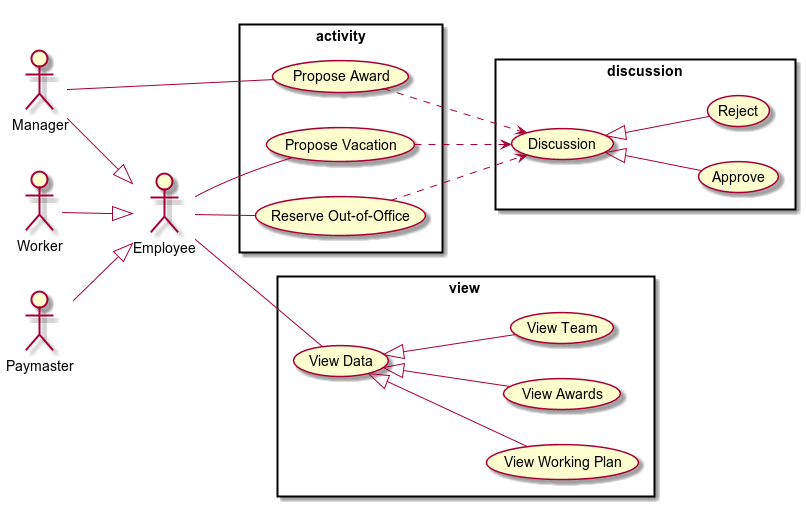
\includegraphics[width=\textwidth]{resources/01_analysis/01_use_cases.png}
    \caption{Диаграма вариантов использования системы}
    \label{fig:01-use-case}
\end{figure}

Приведем здесь подробный разбор вариантов использования системы:
\begin{itemize}
    \item Заявка на выделение премии:
    \begin{enumerate}
        \item \textbf{Пользователь}, выбирает сотрудника, которому необходимо выписать премию. 
        \item \textbf{Система} открывает форму премирования.
        \item \textbf{Пользователь} заполняет данную форму, указывая \textbf{когда} и в каком \textbf{размере} должна быть выплачена 
            премия.
        \item \textbf{Система} проверяет, что пользователь, отправивший заявку, действительно является менеджером по отношению к 
            премируемому сотруднику.
        \item В случае успеха \textbf{система} заносит запись о созданной заявке в базу данных.
        \item В случае ошибки на любом этапе \textbf{система} выводит сообщение об ошибке.
    \end{enumerate}
    \item Заявка на предоставление отпуска:
    \begin{enumerate}
        \item \textbf{Пользователь} нажимает кнопку.
        \item \textbf{Система} открывает форму заявки на предоставление отпуска.
        \item \textbf{Пользователь} заполняет форму.
        \item \textbf{Система} проверяет, что пользователь, отправивший заявку, соответствует работнику, на имя которого запрашивается 
            отпуск.
        \item В случае успеха \textbf{система} заносит запись о созданной заявке в базу данных.
        \item В случае ошибки на любом этапе \textbf{система} выводит сообщение об ошибке.
    \end{enumerate}
    \item Резервирование времени вне офиса:
    \begin{enumerate}
        \item \textbf{Пользователь} нажимает кнопку.
        \item \textbf{Система} открывает форму заявки на резервацию времени вне офиса.
        \item \textbf{Пользователь} заполняет форму.
        \item \textbf{Система} проверяет, что пользователь, отправивший заявку, соответствует работнику, на имя которого отправляется
            заявка.
        \item В случае успеха \textbf{система} заносит запись о созданной заявке в базу данных.
        \item В случае ошибки на любом этапе \textbf{система} выводит сообщение об ошибке. 
    \end{enumerate}
    \item Подтверждение заявки:
    \begin{enumerate}
        \item \textbf{Пользователь} нажимает кнопку.
        \item \textbf{Система} проверяет, что роль пользователя соответствует выполняемой операции:
        \begin{itemize}
            \item Если подтверждается заявка на премию, то пользователь должен иметь роль <<бухгалтер>>.
            \item Если подтверждается заявка на предоставление отпуска, то пользователь должен иметь роль <<менеджер>>.
        \end{itemize}
        \item В случае успеха \textbf{система} обновляет запись о соответствующей заявке в базу данных.
        \item В случае ошибки на любом этапе \textbf{система} выводит сообщение об ошибке. 
    \end{enumerate}
    \item Отклонение заявки:
    \begin{enumerate}
        \item \textbf{Пользователь} нажимает кнопку.
        \item \textbf{Система} проверяет, что роль пользователя соответствует выполняемой операции:
        \begin{itemize}
            \item Если отклоняется заявка на премию, то пользователь должен иметь роль <<бухгалтер>>.
            \item Если отклоняется заявка на предоставление отпуска, то пользователь должен иметь роль <<менеджер>>.
        \end{itemize}
        \item В случае успеха \textbf{система} обновляет запись о соответствующей заявке в базу данных.
        \item В случае ошибки на любом этапе \textbf{система} выводит сообщение об ошибке. 
    \end{enumerate}
\end{itemize}

Доменная модель системы в нашем случае описывается сущностями, представляющими пользователей системы и сущности, с которыми они 
взаимодействуют. Таким образом, модель предметной области в нотации UML будет выглядеть как показано на рисунке \ref{fig:01-domain}.

\begin{figure}[H]
    \centering
    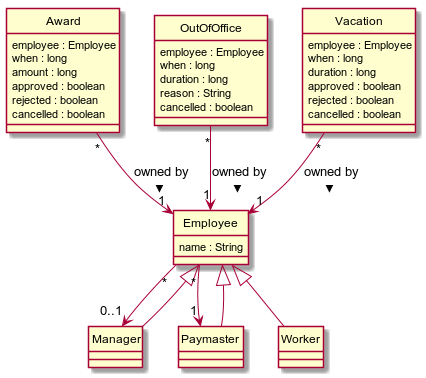
\includegraphics[width=0.8\textwidth]{resources/01_analysis/02_domain.png}
    \caption{Модель предметной области системы}
    \label{fig:01-domain}
\end{figure}

